
\usetikzlibrary{shapes}
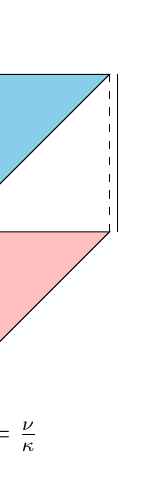
\begin{tikzpicture}[trim left=4.5cm]

        \def\H{1.5}
                \def\W{4}
                        \def\L{5}
                                \draw [fill=SkyBlue] (-1,1,0) --++ (\L,0,0) --++ (0,0,-\W) --++ (-\L,0,0) -- cycle;
                                        % Draw the top plate
                                        % \fill[gray] (-1,1) rectangle ++(7,.1);
                                        % \draw[black] (-1,2) rectangle ++(7,.1);


                                        % Draw the bottom plate
                                        % \fill[gray] (-1,-1.1) rectangle ++(7,.1);
                                        % \draw[black] (-1,-1.1) rectangle ++(7,.1);
                                        \draw [fill=pink] (-1,-1,0) --++ (\L,0,0) --++ (0,0,-\W) --++ (-\L,0,0) -- cycle;

                                               %  % Draw axes
                                               \draw [dashed, thin] (-1, -1, 0) --++ (0, 2, 0);
                                                      \draw [dashed, thin] (\L-1, -1, 0) --++ (0, 2, 0);
                                                             \draw [dashed, thin] (\L-1, -1, -\W) --++ (0, 2, 0);
                                                                    \draw [dashed, thin] (-1, -1, -\W) --++ (0, 2, 0);
                                                                           %\draw [dashed, thin] (-1,0, 0) --++ (\L,0,0) --++ (0,0,-\W) --++ (-\L,0,0) -- cycle;
                                                                           %  % \draw [thin, dashed] (-1,0) -- (6,0);

                                                                           % Add dimensions
                                                                           % \draw [<->] (\L-1+0.1,-1, 0) -- (\L-1+0.1,0,0);
                                                                           % \node[right] at (\L-1+0.1,-0.3,0) {$h$};

                                                                           %\draw [<->] (\L-1+0.1, -1, -\W) -- (\L-1+0.1,1,-\W);
                                                                           \draw [-] (\L-1+0.1, -1, -\W) -- (\L-1+0.1,1,-\W);
                                                                                  % \node[right] at (\L-1+0.1,0.0,-\W) {$d$};
                                                                           % 
                                                                                  % \draw [<->] (-1.1, -1.1, 0) -- (\L-1-0.1,-1.1,0);
                                                                                  % \draw [<->] (\L-1+0.1, -1.1, 0) --++ (0,0,-\W);
                                                                                  % \node[below] at (2.5,-1.1,0) {$L$};
                                                                                  % \node[below] at (\L-1+0.1,-1.1,-\W/2-0.5) {$L$};

                                                                                  % Draw the velocity profile
                                                                                  \draw[->, thick] (-1, 0, 0) -- (-1,0.5,0) node[left] {$y$};
                                                                                         \draw[->, thick] (-1, 0, 0) -- (-0.5,0,0) node [below] {$x$};
                                                                                                \draw[->, thick] (-1, 0, 0) -- (-1,0,-7/4*0.5) node[above] {$z$};

                                                                                                       % Draw the velocity profile
                                                                                                       % \draw[blue,thick,domain=-1:1,samples=200,smooth] plot ({(1-\x*\x)*1.5+0.0}, \x) node[above right] {};
                                                                                                       % \draw[blue,thick,domain=-1:1,samples=200,smooth] plot ({(1-\x*\x)*1.5+0.0}, \x, -\W) node[above right] {$u(y)$};
                                                                                                       % \draw[-,blue,dashed] (0.0,-1) -- (0.0,1);
                                                                                                       % \draw[-,blue,dashed] (0.0,-1,0) --++ (0,0,-\W) --++ (0,2,0) --++ (0,0,\W) -- cycle;
                                                                                                % 
                                                                                                       % \foreach \y in {-0.8,-0.6,...,0.8} {
                                                                                                       %     \draw[-latex,blue] (0.0,\y) -- ({(1-\y*\y)*1.5+0.0},\y);
                                                                                                       %     \draw[-latex,blue] (0.0,\y, -\W) -- ({(1-\y*\y)*1.5+0.0},\y,-\W);
                                                                                                       % }

                                                                                                       % Draw the temperature profile
                                                                                                       \draw[red,thick,domain=-1:1,samples=200,smooth] plot ({3+(1/2*(1-\x)*2-2.5)}, \x);
                                                                                                              \draw[red,thick,domain=-1:1,samples=200,smooth] plot ({3+(1/2*(1-\x)*2-2.5)}, \x, -\W);
                                                                                                                     \draw[-,red,dashed] (2.5,-1,0) --++ (0,0,-\W);
                                                                                                                            \draw[-,red,dashed] (0.5,-1,0) --++ (0,0,-\W) --++ (0,2,0) --++ (0,0,\W) -- cycle;
                                                                                                                            % 
                                                                                                                                   \foreach \y in {-0.8,-0.6,...,0.8} {
                                                                                                                                                  \draw[-latex,red] (0.5,\y) -- ({3+(1/2*(1-\y)*2-2.5)},\y);
                                                                                                                                                             \draw[-latex,red] (0.5,\y, -\W) -- ({3+(1/2*(1-\y)*2-2.5)},\y, -\W);
                                                                                                                                                                    }

                                                                                                                                                                           % Add labels
                                                                                                                                                                           \node[above,red] at (1,1,-\W) {$\theta(y)$};

                                                                                                                                                                                  \node at (2.8,-2.) {$Ra = \frac{\alpha g d^3 \Delta \theta}{\kappa \nu}, \quad Pr = \frac{\nu}{\kappa}$};
                                                                                                                                                                                      \end{tikzpicture}
